$$Agreement \Leftrightarrow Consensus \Leftrightarrow Consistency$$

\paragraph{Atomic broadcast}
\begin{itemize}
    \item Total Order property:

        $p, q$ two correct node and $m, n$ two message $\Rightarrow$ if $p$
        delivers $m$ before $n$ then $q$ delivers $m$ before $n$.

        $\rightarrow $ It's a strong consistency.

    \item No creation of message
    \item No duplication of message (delivered once)
\end{itemize}

This could be useful to have replication because all
database replicas apply updates/queries  in  
the  same  order.

\subsection{Zookeeper}
Zookeeper is a set of data node (\textbf{znodes}) which are organized in a
hierarchical namespace that resembles customary file systems. 
This file system is designed to store \textbf{metadata} and not data.
Zookeeper is a \textsc{CP} for the CAP point of view.

The \textbf{znodes} can be of two types:

\begin{itemize}
	\item \textbf{regular}: clients manipulate regular znodes by creating and deleting them explicitly.
	\item \textbf{ephemeral}: clients can delete them explicitly or let the system remove them automatically when their session terminates.
\end{itemize}

\paragraph{Session}
Client connects  to  Zookeeper  and  initiates  a  session
which allow client to move from one server to another. 
Any server can serve client's requests.

If the server fail, the client library tries to  contact  another  server
before  session  expires.

\paragraph{Consensus}
Zookeeper  can  solve  consensus  (agreement)   for  arbitrary  number  
of  clients.

\subsubsection{Global structure}
\begin{tabular}{m{8cm}m{8cm}}
    \begin{itemize}
        \item Fully replicated (no partitionning)
        \item Use commit log and periodic snapshot to recovery
            on crash
        \end{itemize}
    &
    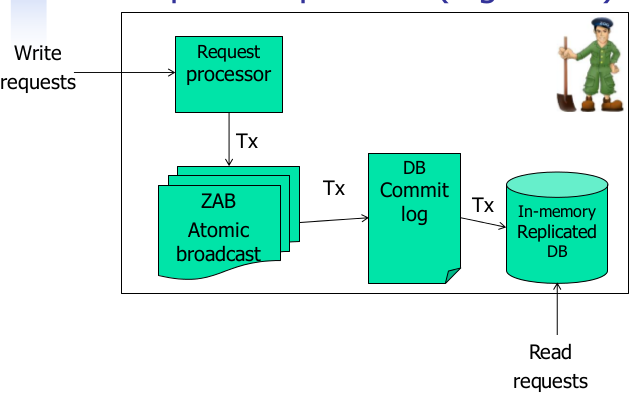
\includegraphics[width=8cm]{img/zookCompo}
\end{tabular}

\subsubsection{Operations}

\begin{tabular}{m{9cm}m{6cm}}
Only full reads and write operations which can 
be asynchronous (concurrent calls allowed and so multiple requests) or synchronous
(no concurrent calls by a single client).
&
    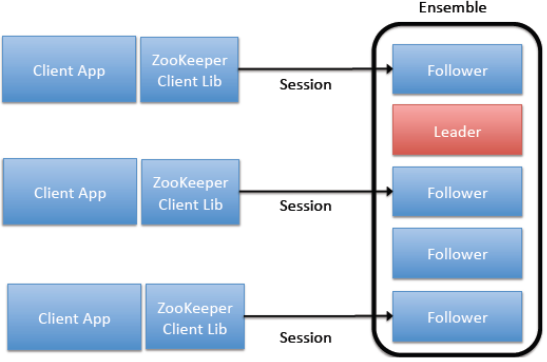
\includegraphics[width=7cm]{img/zook}
\end{tabular}
    \begin{itemize}
        \item \textbf{Write}:
            \begin{tabular}{l}
                \texttt{create(znode, data, flags)}\\
                \texttt{setData(znode, data, version)}\\
                \texttt{delete(znode, version)}\\
                \texttt{sync()}
            \end{tabular}

            \paragraph{Linearizable} Write are linearizable.

            \begin{enumerate}
                \item Write request is forwarded by a follower
                    to the leader
                \item Leader use atomic (total-order) broadcast to
                    disseminate messages

                    $\rightarrow$ use ZAB protocol which support  FIFO/causal  
                    consistency  of  asynchronous  calls. 
                    ZAB tolerate $\frac{n-1}{2}$ failures.
            \end{enumerate}

            \paragraph{ZAB} use a internally elects leader for replica 
            (which is adopted by zookeeper)
            
            \paragraph{Request Processor}
            Upon receiving write request, the leader calculates in what state 
            the system will be after the write is applied and transforms the operation
            in the transactional update. These transactional update are then 
            processed by the ZAB and the DB.
            %TODO slide 64 for 11

        \item \textbf{Read}:
            \begin{tabular}{l}
                \texttt{exist(znode, watch)}\\
                \texttt{getData(znode, watch)}\\
                \texttt{getChildren(znode, watch)}
            \end{tabular}

            \paragraph{Linearizable}
            Read has \textbf{local read} (A  server  serving  a  read  request  might  not  have  been  a  part  of  a  write  
            quorum  of  some  previous  operation). 
            But if \texttt{sync()} is use before each read, we have a \textbf{linearizable read}.

            Indeed, the linearizable read is show as a \textit{slow read}.

            \paragraph{Caching reads}
    \end{itemize}

Leader atomically broadcast updates but read operations is processed
locally.

\paragraph{Flags}

\begin{itemize}
    \item Flags: Regular, Ephemeral, Sequential (  monotonically
        increasing  value  is  appended  to  the  
        name  of  znode)
    \item Version: -­1  to  omit  the  conditional  check  (applies  to
        other  operations  as  well)  
        \item Watch: flag  enables  a  client  to  set  a  watch  on  the
            znode. Watch  is  a  subscription  to  receive  an
            information  from  the  
            Zookeeper  when  this  znode is  changed

            \paragraph{Note}: a  watch  may  be  set  even  if  a  znode
            does  not  exist getData(znode,  watch).  The  client  will
            be  then  informed  when  a  znode is created

\end{itemize}


\subsubsection{Examples}
%TODO slides 51 to 59 for 11


